\chapter{Evaluation}

% Requirements
% * Functional
% * Non-functional
%
% Algorithm
% * Gleichverteilt
% * Umfrage
%
% Implementation
% * scaling
% * ldap connections sind ne bitch
%
% Conclusion

\section{Fitness Score Algorithm}

\subsection{Uniform Distribution of Score Values}
The scores calculated by the fitness score algorithm (see \ref{fitscorealg}) should be distributed uniformly in the complete range of possible values because this does not only generate the best search results, but also is an indicator for the algorithm's fairness.
To test this, one hundred persons have been fed into the system. Each test person has been assigned a random number of skills between zero and 17, with random skill and will levels each. A search for any skill will return a list of up to one hundred persons sorted by their fitness score. The search results for the skills \textit{Atomic Design}, \textit{Datenbanken}, \textit{Funkspots}, \textit{hybris}, \textit{Kommunikation}, \textit{MySQL}, \textit{Sktech} and \textit{Text} have been analyzed because those have the highest number of results (33 each); all results can be found in table \ref{alldatatable}. Ideally, the scores in each result list decline linearily from one to zero. The ideal value for the $n$-th result value is:
\[
	v_{Ideal}(n) = 1 - \frac{n}{33}
\]

The distribution of the score values for every respective search is shown in figure \ref{fig:dist-raw}.
Figure \ref{fig:dist-avg} illustrates the average of all eight scores for each postion in the search result lists, the maximum value found at this position, and the respective minimum value.
It shows that the average score declines linearily, which means that the score values are distributed uniformly thorough the result lists. In figure \ref{fig:dist-raw}, every result function shows a variance from the ideal value; the average value in figure \ref{fig:dist-avg}, however, deviates signifitantly less from the ideal than any of the isolated data rows. This leads to the conclusion that the drift from the ideal that occurs when observering one single set of data for one specific search is based on the small amount of examined values (33 data points). The average fitness score shows an average error of approx. 6\% (see figure \ref{fig:dist-err}). The maximum error in the given set of data is 27\%.
This leads to the conclusion that the fitness score algorithm generates uniformly distributed score values with an acceptable error.\\
Interestingly, the maximum error seems to have a declining trend; the small amount of examined data does not provide a solid basis for assumptions about whether there is a systematic reason for this, and, if so, whether it could have a negative impact on the proper working of the system. Unfortunately, there is no authentic usage data yet, so that this question will remain unanswered and might be subject to further research.

\begin{figure}[H]
    \centering
    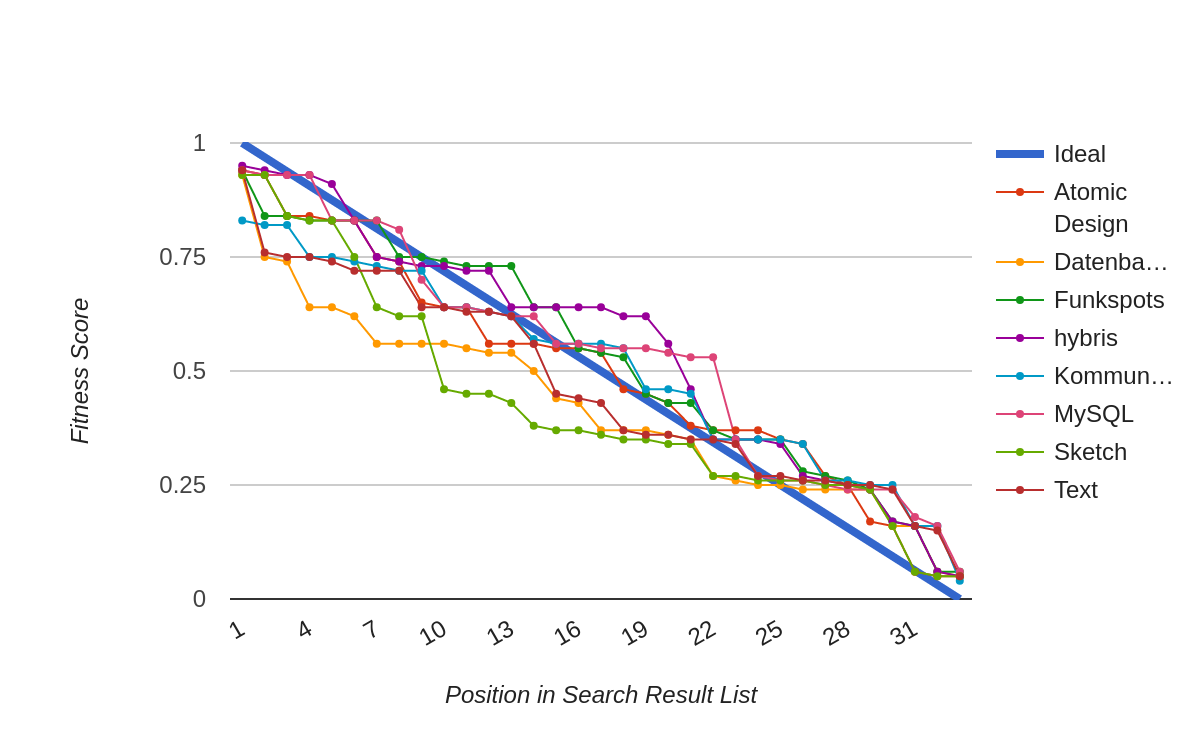
\includegraphics[width=\textwidth]{images/dist_raw.png}
    \caption[Diagram: Fitness Score Distribution (Raw)]{All search results and the ideal value.}
    \label{fig:dist-raw}
\end{figure}

\begin{figure}[H]
    \centering
    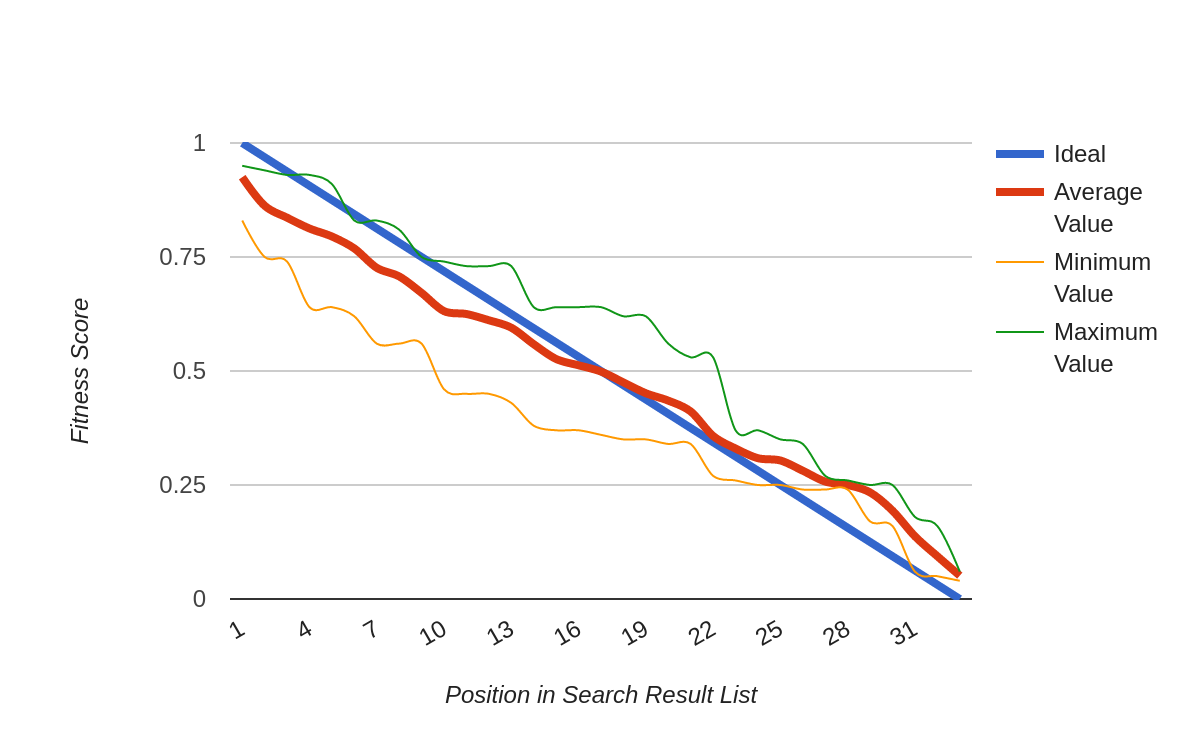
\includegraphics[width=\textwidth]{images/dist_avg.png}
    \caption[Diagram: Fitness Score Distribution (Processed)]{Average, maximum and minimum score for earch position in the respective search result list.}
    \label{fig:dist-avg}
\end{figure}

\begin{figure}[H]
    \centering
    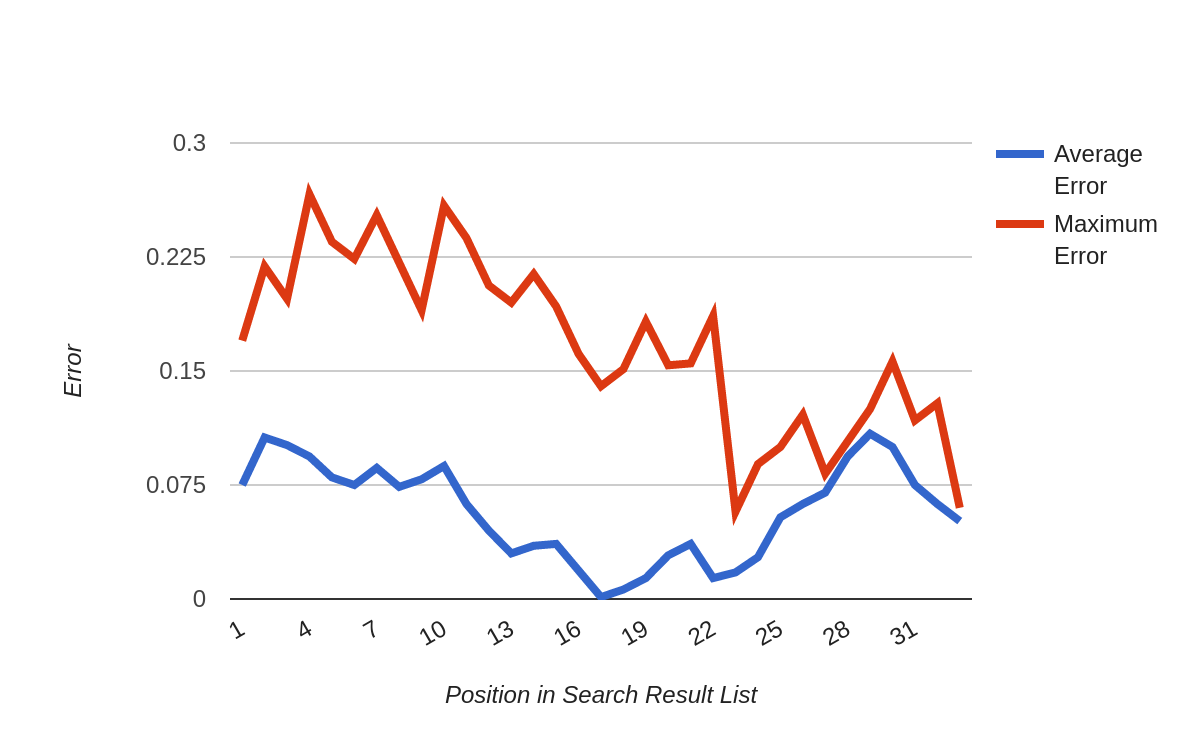
\includegraphics[width=\textwidth]{images/dist_error.png}
    \caption[Diagram: Fitness Score Distribution (Error Rates)]{Average and maximum error (Difference between respective score value and the ideal value).}
    \label{fig:dist-err}
\end{figure}

\begin{table}[H]
\centering
\resizebox{\textwidth}{!}{
\rotatebox{-90}{
  \begin{tabular}{l||c|c|c|c|c|c|c|c|c||c|c|c||c|c}
	  No. & $v_{Ideal}$ & A.D. & DBs & Funk. & hybris & Kom. & MySQL & Sketch & Text & Mean Value & Min. Val. & Max. Val. & Mean Error & Max. Error\\
	  \hline
	  1 & 1 & 0.94 & 0.93 & 0.94 & 0.95 & 0.83 & 0.94 & 0.93 & 0.94  &  0.925 & 0.83 & 0.95  &  0.075 & 0.17\\
 	 2 & 0.96875 & 0.93 & 0.75 & 0.84 & 0.94 & 0.82 & 0.93 & 0.93 & 0.76  &  0.8625 & 0.75 & 0.94  &  0.10625 & 0.21875\\
 	 3 & 0.9375 & 0.84 & 0.74 & 0.84 & 0.93 & 0.82 & 0.93 & 0.84 & 0.75  &  0.83625 & 0.74 & 0.93  &  0.10125 & 0.1975\\
 	 4 & 0.90625 & 0.84 & 0.64 & 0.83 & 0.93 & 0.75 & 0.93 & 0.83 & 0.75  &  0.8125 & 0.64 & 0.93  &  0.09375 & 0.26625\\
 	 5 & 0.875 & 0.83 & 0.64 & 0.83 & 0.91 & 0.75 & 0.83 & 0.83 & 0.74  &  0.795 & 0.64 & 0.91  &  0.08 & 0.235\\
 	 6 & 0.84375 & 0.83 & 0.62 & 0.83 & 0.83 & 0.74 & 0.83 & 0.75 & 0.72  &  0.76875 & 0.62 & 0.83  &  0.075 & 0.22375\\
 	 7 & 0.8125 & 0.75 & 0.56 & 0.83 & 0.75 & 0.73 & 0.83 & 0.64 & 0.72  &  0.72625 & 0.56 & 0.83  &  0.08625 & 0.2525\\
 	 8 & 0.78125 & 0.74 & 0.56 & 0.75 & 0.74 & 0.72 & 0.81 & 0.62 & 0.72  &  0.7075 & 0.56 & 0.81  &  0.07375 & 0.22125\\
 	 9 & 0.75 & 0.65 & 0.56 & 0.75 & 0.73 & 0.72 & 0.7 & 0.62 & 0.64  &  0.67125 & 0.56 & 0.75  &  0.07875 & 0.19\\
 	 10 & 0.71875 & 0.64 & 0.56 & 0.74 & 0.73 & 0.64 & 0.64 & 0.46 & 0.64  &  0.63125 & 0.46 & 0.74  &  0.0875 & 0.25875\\
 	 11 & 0.6875 & 0.64 & 0.55 & 0.73 & 0.72 & 0.64 & 0.64 & 0.45 & 0.63  &  0.625 & 0.45 & 0.73  &  0.0625 & 0.2375\\
 	 12 & 0.65625 & 0.56 & 0.54 & 0.73 & 0.72 & 0.63 & 0.63 & 0.45 & 0.63  &  0.61125 & 0.45 & 0.73  &  0.045 & 0.20625\\
 	 13 & 0.625 & 0.56 & 0.54 & 0.73 & 0.64 & 0.62 & 0.62 & 0.43 & 0.62  &  0.595 & 0.43 & 0.73  &  0.03 & 0.195\\
 	 14 & 0.59375 & 0.56 & 0.5 & 0.64 & 0.64 & 0.57 & 0.62 & 0.38 & 0.56  &  0.55875 & 0.38 & 0.64  &  0.035 & 0.21375\\
 	 15 & 0.5625 & 0.55 & 0.44 & 0.64 & 0.64 & 0.56 & 0.56 & 0.37 & 0.45  &  0.52625 & 0.37 & 0.64  &  0.03625 & 0.1925\\
 	 16 & 0.53125 & 0.55 & 0.43 & 0.55 & 0.64 & 0.56 & 0.56 & 0.37 & 0.44  &  0.5125 & 0.37 & 0.64  &  0.01875 & 0.16125\\
 	 17 & 0.5 & 0.54 & 0.37 & 0.54 & 0.64 & 0.56 & 0.55 & 0.36 & 0.43  &  0.49875 & 0.36 & 0.64  &  0.00125 & 0.14\\
 	 18 & 0.46875 & 0.46 & 0.37 & 0.53 & 0.62 & 0.55 & 0.55 & 0.35 & 0.37  &  0.475 & 0.35 & 0.62  &  0.00625 & 0.15125\\
 	 19 & 0.4375 & 0.45 & 0.37 & 0.45 & 0.62 & 0.46 & 0.55 & 0.35 & 0.36  &  0.45125 & 0.35 & 0.62  &  0.01375 & 0.1825\\
 	 20 & 0.40625 & 0.43 & 0.36 & 0.43 & 0.56 & 0.46 & 0.54 & 0.34 & 0.36  &  0.435 & 0.34 & 0.56  &  0.02875 & 0.15375\\
 	 21 & 0.375 & 0.38 & 0.35 & 0.43 & 0.46 & 0.45 & 0.53 & 0.34 & 0.35  &  0.41125 & 0.34 & 0.53  &  0.03625 & 0.155\\
 	 22 & 0.34375 & 0.37 & 0.27 & 0.37 & 0.35 & 0.35 & 0.53 & 0.27 & 0.35  &  0.3575 & 0.27 & 0.53  &  0.01375 & 0.18625\\
 	 23 & 0.3125 & 0.37 & 0.26 & 0.35 & 0.35 & 0.35 & 0.35 & 0.27 & 0.34  &  0.33 & 0.26 & 0.37  &  0.0175 & 0.0575\\
 	 24 & 0.28125 & 0.37 & 0.25 & 0.35 & 0.35 & 0.35 & 0.27 & 0.26 & 0.27  &  0.30875 & 0.25 & 0.37  &  0.0275 & 0.08875\\
 	 25 & 0.25 & 0.35 & 0.25 & 0.35 & 0.34 & 0.35 & 0.26 & 0.26 & 0.27  &  0.30375 & 0.25 & 0.35  &  0.05375 & 0.1\\
 	 26 & 0.21875 & 0.34 & 0.24 & 0.28 & 0.27 & 0.34 & 0.26 & 0.26 & 0.26  &  0.28125 & 0.24 & 0.34  &  0.0625 & 0.12125\\
 	 27 & 0.1875 & 0.27 & 0.24 & 0.27 & 0.26 & 0.26 & 0.25 & 0.25 & 0.26  &  0.2575 & 0.24 & 0.27  &  0.07 & 0.0825\\
 	 28 & 0.15625 & 0.25 & 0.24 & 0.26 & 0.25 & 0.26 & 0.24 & 0.25 & 0.25  &  0.25 & 0.24 & 0.26  &  0.09375 & 0.10375\\
 	 29 & 0.125 & 0.17 & 0.24 & 0.24 & 0.24 & 0.25 & 0.24 & 0.24 & 0.25  &  0.23375 & 0.17 & 0.25  &  0.10875 & 0.125\\
 	 30 & 0.09375 & 0.16 & 0.16 & 0.17 & 0.17 & 0.25 & 0.24 & 0.16 & 0.24  &  0.19375 & 0.16 & 0.25  &  0.1 & 0.15625\\
 	 31 & 0.0625 & 0.06 & 0.16 & 0.16 & 0.16 & 0.16 & 0.18 & 0.06 & 0.16  &  0.1375 & 0.06 & 0.18  &  0.075 & 0.1175\\
 	 32 & 0.03125 & 0.05 & 0.06 & 0.06 & 0.06 & 0.16 & 0.16 & 0.05 & 0.15  &  0.09375 & 0.05 & 0.16  &  0.0625 & 0.12875\\
 	 33 & 0 & 0.05 & 0.05 & 0.06 & 0.05 & 0.04 & 0.06 & 0.05 & 0.05  &  0.05125 & 0.04 & 0.06  &  0.05125 & 0.06\\
  \end{tabular}
}}
\caption[Fitness Score Distribution (Raw Test Data)]{Fitness score values that have been selected for this test.}
\label{alldatatable}
\end{table}

\newpage

\subsection{Fitness Score Algorithm vs. Human Estimations}
The algorithm is supposed to calculate a person's fitness so that its results match the ratings estimated by other employees. To validate that
the chosen approach is capable of this, a set of fictional employees has been rated by both the algorithm and human beings. The respective estimations have been compared to analyze if there is a configuration of weigthing parameters $w_{as}$, $w_{aw}$, $w_{ss}$ and $w_{sw}$ that make the algorithm produce scores that are
congruent to the estimations made by the rating persons.

\subsubsection{Examined Test Records}
For this test, five test persons will be examined: \textit{Alice}, \textit{Bob}, \textit{Charlie}, \textit{Donald} and \textit{Erika}. Each of this persons has different skill and will levels for the abilities \textit{Java}, \textit{AEM}, \textit{Ruby} and \textit{.NET}. The fitness scores that will be collected and examined focus on the scenario that a potential user searches for the skills \textit{Java} and \textit{AEM}.
\begin{table}[H]
\centering
  \begin{tabular}{l||c|c|c|c}
		Test Record  & Java & AEM & Ruby & .NET\\
		\hline
		Alice   & 3, 3   & 2, 3  & 0, 1   & 2, 2 \\
		Bob     & 2, 1   & 3, 0  & 2, 0   & 3, 3 \\
		Charlie & 1, 3   & 0, 2  & 1, 2   & 2, 3 \\
		Donald  & 1, 2   & 2, 1  & 1, 2   & 2, 1 \\
		Erika   & 1, 0   & 0, 1  & 3, 2   & 3, 1 \\
  \end{tabular}
\caption[Survey: Test Record Overview]{Skill and will levels of the persons presented in the survey. Notation: skill level, will level}
\end{table}

\newpage
\subsubsection{Survey}
A random group of 161 employees (35\% of SinnerSchrader's staff) have been presented a survey using \textit{Google Forms}\footnote{https://forms.google.com}.
In total, 41 persons have given their responses in a timeframe of 72 hours.
The survey consisted of two sections: the estimation of the test persons' fitness scores and the evaluation of the weighting of the factors included in the algorithm. To collect the personal estimations regarding the test records' fitness, the test subjects have been presented \textit{Lickert Items} using a scale form one (``does not fit at all'') to five (``perfect match''). As table \ref{tab:scoretrans} shows, values on this scale can easily be translated into the corresponding fitness score. The results of the survey are shown in table \ref{tab:survey_raw}\footnote{Values have been rounded off to two significant digits.} and figure \ref{survey_raw}.
\begin{table}[H]
\centering
\begin{tabular}{l||c|c|c|c|c}
	Survey Rating & 1 & 2    & 3   & 4    & 5\\
	\hline
	Fitness Score & 0 & 0.25 & 0.5 & 0.75 & 1\\
\end{tabular}
\caption[Survey: Rating to Fitness Score]{Conversion from survey rating to fitness score.}
\label{tab:scoretrans}
\end{table}

\begin{table}[H]
\centering
\begin{tabular}{l||c|c|c|c|c|c||c|c}
Test Record & 1  & 2  & 3  & 4  & 5  & - & Mean & $f$ \\
\hline
Alice       & 0  & 0  & 0  & 15 & 26 & 0 & 4.63 & 0.91 \\
Bob         & 5  & 26 & 9  & 1  & 0  & 0 & 2.15 & 0.27 \\
Charlie     & 1  & 14 & 23 & 3  & 0  & 0 & 2.68 & 0.42 \\
Donald      & 0  & 10 & 27 & 3  & 0  & 1 & 2.83 & 0.46 \\
Erika       & 32 & 70 & 0  & 2  & 0  & 0 & 1.31 & 0.08 \\
\end{tabular}
\caption[Survey: Estimated Fitness Scores]{Fitness scores estimated by 41 test subjects}
\label{tab:survey_raw}
\end{table}

\begin{figure}[H]
    \centering
    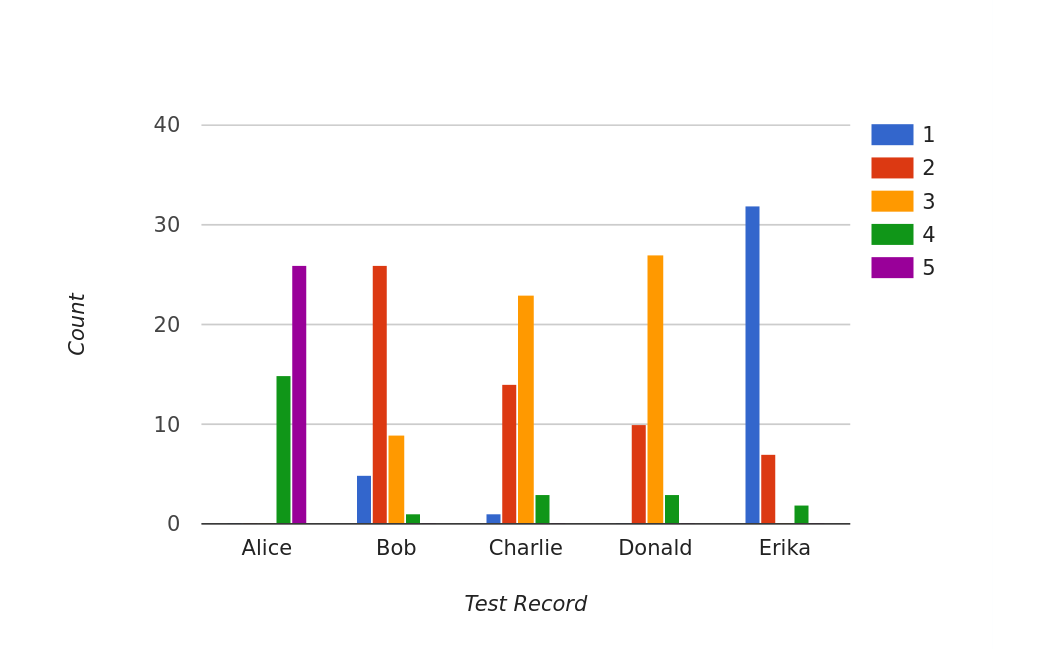
\includegraphics[width=\textwidth]{images/survey_raw.png}
    \caption[Diagram: Survey Data]{Data collected in the survey.}
    \label{survey_raw}
\end{figure}

Furthermore, the participants were asked to rate the importance of the four factors included in the algorithm (see \ref{fitscorealg}), namely the person's average level of skill and will in the searched items, and their respective specialization in the items, on a scale from one (``not important'') to five (``very important''). The results illustrated in table \ref{tab:survey_weight} show that all factors are valued nearly equally important.
\begin{table}[H]
\centering
\begin{tabular}{l||c|c|c|c|c|c||c}
Factor & 1  & 2  & 3  & 4  & 5  & -\footnote{No Response} & Mean \\
\hline
Avgerage Skill Level in Searched Items & 1 & 3 & 10 & 16 & 11 & 0 & 3.80\\
Avgerage Will Level in Searched Items & 0 & 1 & 8 & 16 & 16 & 0 & 4.15\\
Specialization in Searched Items (Skill Levels) & 3 & 5 & 17 & 12 & 4 & 0 & 3.22\\
Specialization in Searched Items (Will Levels) & 1 & 0 & 11 & 22 & 5 & 2 & 3.77\\
\end{tabular}
\caption[Survey: Estimated Importance of Weighting Factors]{The importance of the four factors included in the fitness score algorithm as estimated by 41 test subjects.}
\label{tab:survey_weight}
\end{table}


Using this data to calculate the weighting parameters $w_{as}$, $w_{aw}$, $w_{ss}$ and $w_{sw}$ results in the following values:
\begin{table}[H]
\centering
\begin{tabular}{l||c|c|c|c}
Parameter & $w_{as}$ & $w_{aw}$ & $w_{ss}$ & $w_{sw}$\\
\hline
Weight & 25.44\% & 27.78\% & 21.55\% & 25.23\% \\
\end{tabular}
\caption[Survey: Resulting Weighting Parameters]{Weighting parameters based on the collected data.}
\end{table}

\subsubsection{Comparison}
To benchmark its results, the fitness score algorithm has been configured to use the weighting score parameters based on the data collected in the survey.
The fitness rated by the algorithm will be called $f_a$; the fitness estimated by the test subjects will called $f_s$.
The results illustrated in table \ref{tab:survey_raw} and figure \ref{survey:compare} show that the estimated and the calculated scores correlate with an average error of 9.4\% and a maximum error of 11.1\%. Since the data colleced in the survey is likely to be inaccurate because of the scale's low resolution of five distinct options and due to the small number of test records, these results should be taken with a grain of salt.

\begin{table}[H]
\centering
\begin{tabular}{l||c|c|c}
Test Record & $f_a$ & $f_s$ & $\Delta_{f}$ \\
\hline
Alice       & 0.82 & 0.91 & 0.09\\
Bob         & 0.45 & 0.27 & 0.18\\
Charlie     & 0.47 & 0.42 & 0.05\\
Donald      & 0.5  & 0.46 & 0.04\\
Erika       & 0.19 & 0.08 & 0.11\\
\end{tabular}
\caption[Survey: Comparison of Algorithm and Survey]{Comparison of the algorithms results and the scores collected in the survey.}
\label{tab:survey_raw}
\end{table}

\begin{figure}[H]
    \centering
    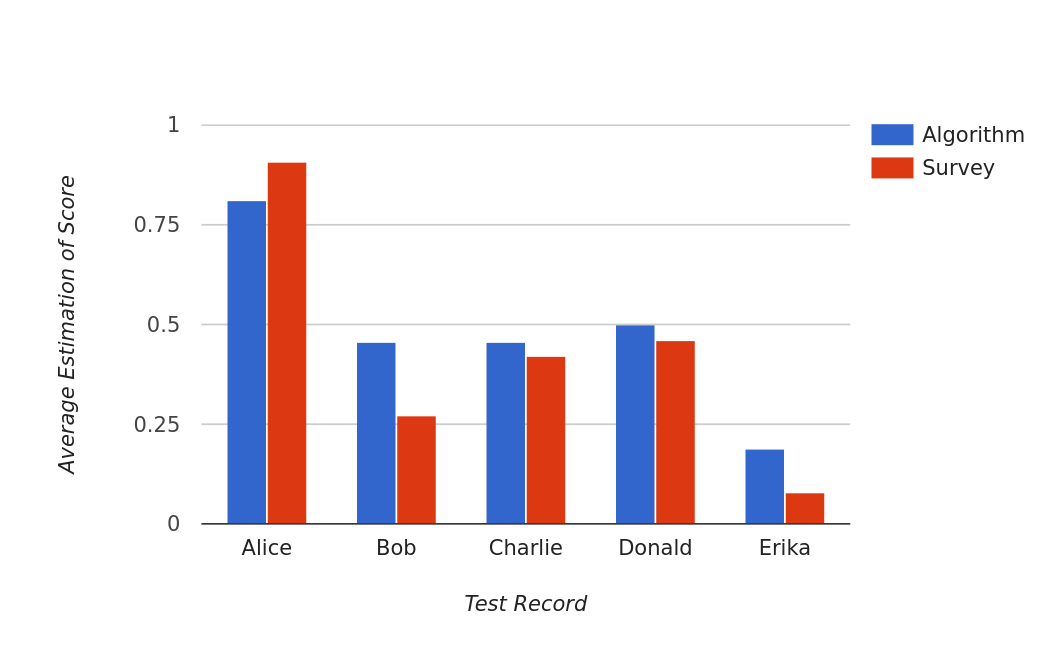
\includegraphics[width=\textwidth]{images/survey_vs_alg.png}
    \caption[Diagram: Comparison of Survey and Algorithm]{Comparison of estimated scores collected in the survey and generated by the algorithm.}
    \label{survey:compare}
\end{figure}

\subsubsection{Refining the Fitness Score Algorithm}
The weighting parameters generated from the survey data are all in the order of 25\%; in fact, setting all parameters to 0.25 will not cause any significant change in the algorithms error rate\footnote{It would reduce the average error from 9.46\% to 9.43\% and the maximum error from 11.07\% to 10.7\%.}, but it will result in all factors being considered equally important and thus reduce the algorithm's complexity.
Furthermore, settings the factors to $w_{as} = w_{aw} = w_{ss} = w_{sw} = 0.25$ means they could be eliminated in the fitness score function\footnote{Definitions can be found in \ref{fitscorealg}.}:

\begin{gather*}
  f = \frac{w_{as} \cdot a_s}{max(V)} + \frac{w_{aw} \cdot a_w}{max(V)} + w_{ss} \cdot s_s + w_{sw} \cdot s_w
\end{gather*}
\begin{gather*}
	\Rightarrow f = \frac{a_s + a_w}{4 max(V)} + \frac{s_s + s_w}{4}
\end{gather*}

\subsubsection{Conclusion}
Comparing the algorithm's results with the values collected in the survey has shown that the algorithmic approach can be used to generate
suitable ratings of an employee's fitness into a specific set of searched skills. The analysis of the collected data has also demonstrated that the algorithm
does not need to include weighting parameters since the test subjects perceive all factors to be equally important. Nonetheless, the factors will not be excluded from the algorithm's implemenation since having the possibility to tweak its working might come in handy if the future day to day use of the application reveals other requirements for the weighting.

\newpage
\section{Implementation}
\subsection{Scalability}
\label{scale}
A software system has to be able to scale according to the number of its users in order to be future-proof, as the current trend to dynamically scalable cloud solutions and server-less web architectures highlights \cite{allthecloud}. There are two concepts of preparing an application for a higher workload: vertical scaling and horizontal scaling. Vertical scaling is done by providing more resources, e.g. memory and CPU power, to the machines running the application. Horziontal scaling, however, means setting up more machines providing the same service, so that the workload can be distributed between them \cite{hvscale}. In contrast to vertical scaling, horizontal scaling has vital advantages: the application will be more robust since the crashing of one machine can be compensated by others \cite{fedi}, the capacity of the system can, theoretically, be unlimited, and it is cheaper because virutal machines running the service can be created dynamically if needed and then be destroyed in times of low workload, whereas the resources given to a machine that has been scaled vertically will remain unused.

\begin{figure}[!htp]
    \centering
    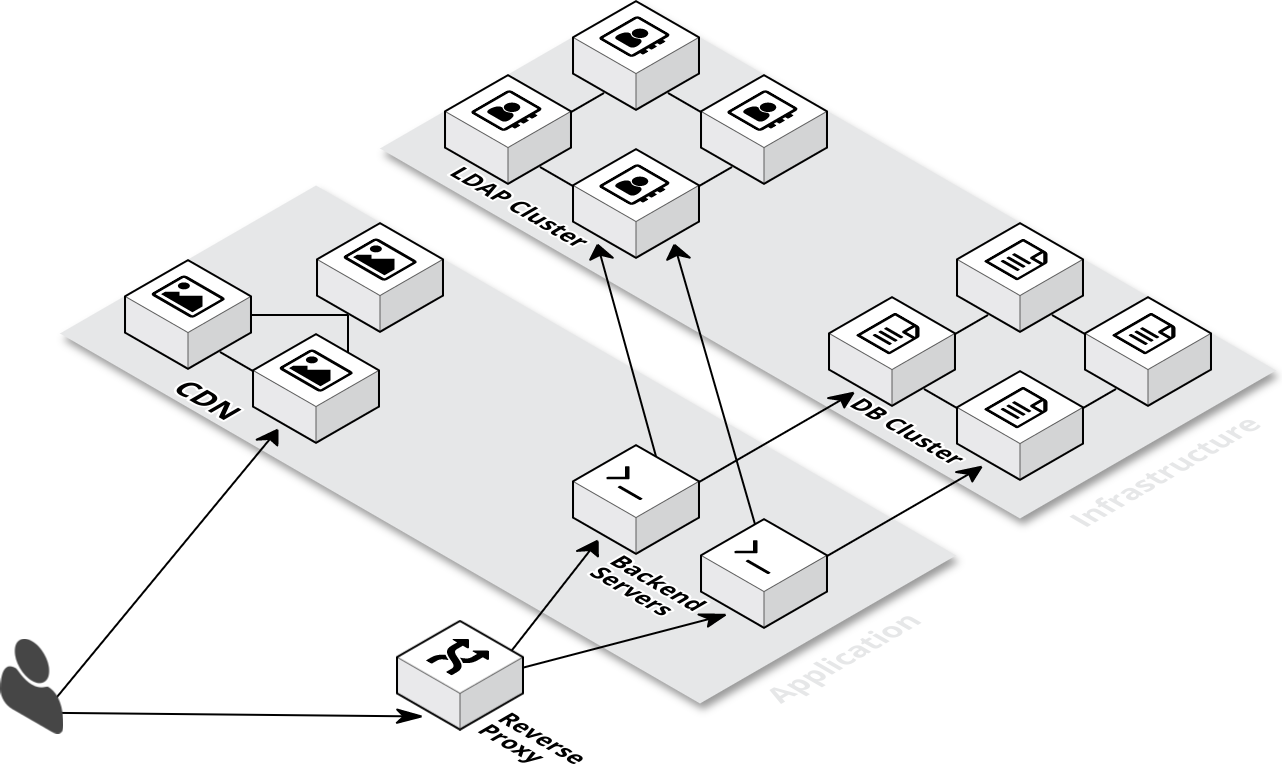
\includegraphics[width=0.75\textwidth]{images/system_architecture_scaled.png}
    \caption[Illustration: Scaled System Architecture]{A possible approach to scale the system using multiple backend servers, a CDN, and multiple clustered database and ldap servers. Created with \textit{https://cloudcraft.co}.}
    \label{scaleup}
\end{figure}

\newpage
\subsubsection{MongoDB}
MongoDB is meant to be scaled horizontally and supports the adding of new instances to a running cluster of databases out of the box \cite[p. 19]{MongoGuide}. So, new machines running the database as a cluster will be created, if needed. As shown in \ref{scaleup}, the backend servers can be connected to any of the database servers in order to request data. If the demanded document is not found on the instance the backend is connected to, MongoDB will handle the lookup in the cluster. To the application, the cluster is completely transparent and appears as if it was one machine.

\subsubsection{LDAP}
The LDAP servers\footnote{SinnerSchrader is running \textit{OpenLDAP} (http://www.openldap.org)} can also be run as a cluster in order to improve response times and prevent data loss by replicating the stored information \cite{ldapscale}. In fact, the LDAP is currently being provided by six servers that represent the service. As illustrated in figure \ref{scaleup}, the backend servers can connect to any of the LDAP servers; the data replication and synchronization is handled transparently.

\subsubsection{Static Content}
The static content like HTML, CSS and JS files, that altogether represent the frontend, are
served by the reverse proxy web server. In the event of an increasing number of requests that cannot be handled by the single server, a \textit{Content Delivery Network} (CDN) could be deployed. A CDN is a network of webservers that provide static content and large files. The reverse proxy would redirect the URLs for those files, so that the users' browsers will connect directly to said network in order to retrieve the assets.

\subsubsection{Backend}
The backend application itself does not save any data on the machine it is running on, but connects a database server (see \ref{impl:be}). As a result, any number of backend instances can be set up. In contrast to the other services, the backend servers do not have to synchronize. In order to receive HTTP requests, the reverse proxy must be configured so that it redirects API calls to the backend servers. This is called \textit{load balancing} and is supported by many modern web servers such as \textit{nginx}\footnote{https://www.nginx.com/resources/wiki/}, \textit{Apache}\footnote{https://httpd.apache.org/} and \textit{Tomcat}\footnote{http://tomcat.apache.org/}.

\newpage

\subsubsection{Conclusion}
In theory, the application should be able to scale according to the number of its users. Practically, only the running of multiple backend and LDAP servers has been tested successfully. Running multiple database instances has not been tested; since MongoDB has been designed to be horizontally scalable and comes to use in various companies like
\textit{Github}\footnote{https://www.mongodb.com/presentations/mongosv-2012/mongodb-analytics-github},
\textit{eBay}\footnote{https://www.mongodb.com/presentations/mongodb-ebay}, and
\textit{Otto}\footnote{https://www.mongodb.com/industries/retail}, it can be assumed that this can be done successfully for this application, too.
Deploying a CDN that serves the static content has not been evaluated, as the implementation of the frontend was not part of this thesis, but has been worked on by Strecker \cite{strecker}.

\subsection{Response Times}
\label{resptime}
As defined in \ref{require_times}, the application should need less than one second of response time between the user pressing the search button and the
displaying of the search results. The response times of the corresponding API endpoint have been measured and can be found in table \ref{tab:responsetimes}.
The average response time of the backend is 28ms, the maximum in the test data is 44ms.

\begin{table}[H]
\centering
  \begin{tabular}{l|c|c|}
		Request Parameters                    & Response Times (in ms)                & Mean\\
		\hline
		No parameters               & 26, 28, 27, 40, 27, 33, 28, 29, 26, 29 & 29\\
		Specific Skill              & 32, 40, 30, 32, 26, 24, 28, 44, 33, 32 & 32\\
		Specific Location           & 27, 26, 26, 25, 26, 36, 26, 22, 21, 25 & 26\\
		Specific Skill and Location & 36, 24, 23, 21, 22, 24, 33, 20, 30, 21 & 25\\
  \end{tabular}

\caption[API Response Times]{Measured response times of the api endpoint for the search function.}
\label{tab:responsetimes}
\end{table}

Measurements of a prototypical stage of the frontend using \textit{Google Chrome's} built-in profiling tools showed a total response time, that is sending the HTTP request to the API, waiting for the response, parsing the response, and rendering the results, of approximately 90ms on average. The maximum response time was 106ms.

Those results show that the API is capable of serving the requests quickly enough to reach the goal of a response time under one second. The outcome of the profiling of the prototypical frontend suggest that it might even be possible to attain a total loading time of under 100ms; according to Kearney, this is would result in the users percieving the interaction with the system as immediate \cite{RAIL}, which enhances the overall user experience.

\newpage

\section{Meeting the Requirements}
In \ref{requirements}, a set of functional and non functional requirements has been defined. The backend application that has been designed and implemented has to meet those requirements, and it does: the API supports the creation of user profiles that then can be retrieved, the skills in those profiles can be edited by the profile's owner only, everybody can search for profiles of persons that offer specific skills (see table \ref{swaggertable}). The application was designed to be accessible to all employees, thus it is implemented as a web application that can be opened by any internet enabled device. New skills can be fed into the system so that people can add them to their profiles. \newline
The non functional requirements included scalability, low response times, the supported devices and browsers.
As shown in \ref{scale}, scalability has been partially evaluated, whereas services that the application relies on such as MongoDB and LDAP were assumed to be scalable in this architecture as comparable systems have already shown. The response times have been evaluated in \ref{resptime}; the results and tests with and prototypical stage of the frontend show that the application is capable of delivering the requested inforamtion in significantely less time than defined.
The requirements for supported devices and browsers, however, could not be evaluated since the determinative factor for those is the implementation of the frontend which has not been part of this thesis and will be evaluated by Strecker \cite{strecker}.
